\Titular%
{O efecto Dzhanibekov}%
{Martín Alberto Häderli Revuelta}%
{divulgacion}%
{Un fenómeno físico que conecta aos mongois, Euler e... a fin do Mundo?}%

\begin{refsection}
\begin{multicols}{2}


É o turno de adentrarse nunha das conexións máis curiosas da física: como
poderían conectarse o Imperio mongol, a fin da carreira espacial entre a URSS e
os EUA, a apocalipse e, como non, Euler? Prepárate, porque quizais terminamos
dando... algunha que outra volta; imos, pois, falar do \textit{\textbf{Efecto
Dzhanibekov}}.

\subsection*{A historia}

O punto de partida da nosa aventura é o 11 de febreiro de 1985, no medio da que
é popularmente recoñecida como a etapa máis tensa da Guerra Fría. Os sistemas
de control da estación espacial soviética Salyut 7 fallaron e perdeuse o
contacto coa nave. Ao non haber tripulantes nese momento, a estación espacial
comezou a vagar sen control, rotando sobre o seu eixo axial, que é o eixo
principal con menor momento de inercia. Isto foi crucial, dado que segundo a
dinámica do corpo ríxido o movemento dun corpo que xira sobre un dos seus eixos
principais é estable sempre e cando teñan asociados ou o menor ou o maior
momento de inercia (recordaremos isto máis adiante). Consecuentemente, aínda
existía unha pequena posibilidade de iniciar unha misión espacial para tentar
reparar os fallos e recuperar o control sobre a Salyut 7. Porén, era necesario
recrutar os cosmonautas adecuados e aí é onde entra en escena o noso
protagonista: \textbf{Vladimir Aleksandrovich Krysin}.\\

\begin{centering}
    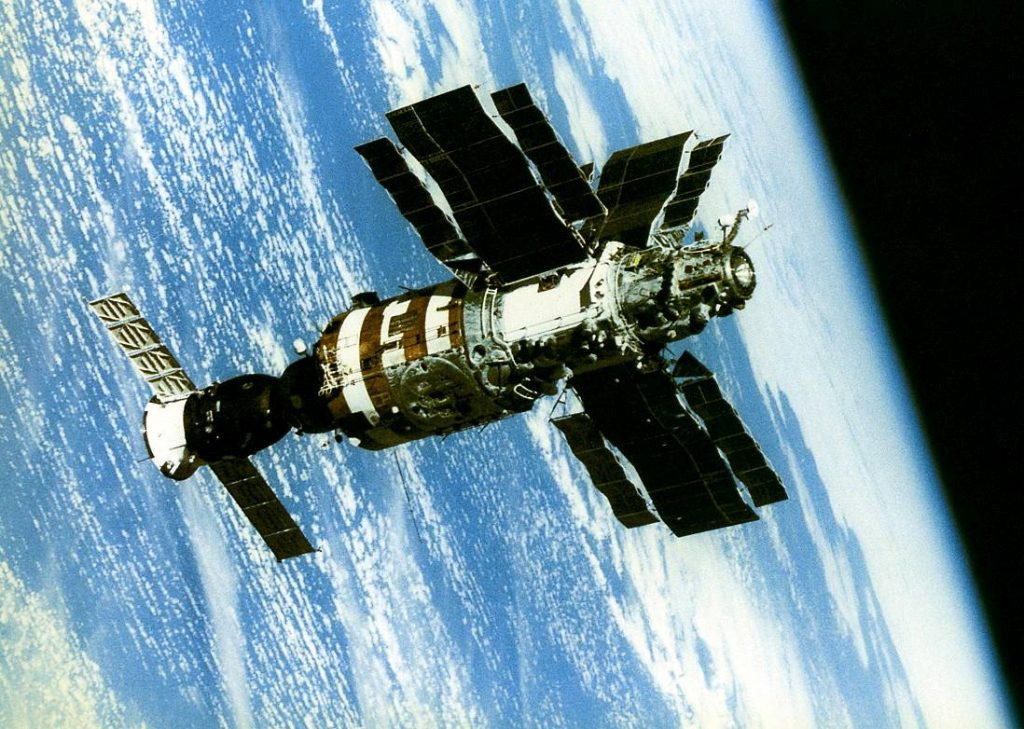
\includegraphics[width=0.8\linewidth]{revistas/002/imaxes/img1.jpg}
    \captionof{figure}{Estación espacial Salyut 7.}
    \label{fig:salyut}
\end{centering}\vspace{10pt}

Vladimir naceu no actual Uzbekistán e estudou física na Universidade de
Leningrado para posteriormente graduarse como instructor de voo nas Forzas
Aéreas Soviéticas, onde logo foi seleccionado como cosmonauta. Á idade de 22
anos casou con Liliya Dzhanibekova, descendente directa de Janibeg, un líder
medieval dun dos reinos que quedaron logo da disolución do Imperio Mongol. Como
consecuencia de que o pai de Liliya non tiña fillos varóns, Vladimir decidiu
adquirir o apelido da súa muller como forma de honrar aos seus ancestros e
continuar coa liña de descendencia, pasando a chamarse \textbf{Vladimir
Dzhanibekov}. Durante os seguintes anos, Dzhanibekov participou en cinco
misións espaciais, e foi nesta última onde descubriu o efecto que toma o seu
apelido, mais non nos adiantemos.

Regresemos ata o 6 de xuño de 1985 no cosmódromo de Baikonur, actual
Kazakhstán. Ás 06:39:52 dese mesmo día despegou de alí a nave Soyuz-U2, a bordo
con Dzhanibekov e un enxeñeiro de voo co fin de recuperar a Salyut 7. Dado o
feito de que o xiro da estación era estable, os soviéticos puideron facer as
manobras para se aproximaren o suficiente á nave e facer coincidir as rotacións
conseguindo finalmente recuperar o control da estación espacial, así
converténdose esta nunha das fazañas máis notables da astronáutica. Unha vez
comprobaron que o aire era respirable, os cosmonautas entraron na estación e
comezaron a facer as reparacións necesarias. Dezanove días despois, ocorrería o
achado. Mentres Dzhanibekov desempacaba a subministración do envío espacial
Progress-24, unha porca con dúas ás saíu xirando do seu sitio. O problema viu
cando logo duns segundos, este elemento cambiou de orientación e puxérase a
xirar noutro sentido como se de maxia negra se tratase. O cambio de orientación
na rotación dun obxecto que en principio non estaba a xirar nese eixo é o que
actualmente se denomina como \textbf{efecto Dzhanibekov} ou tamén
\textbf{teorema da raqueta de tenis}.\\

\begin{centering}
    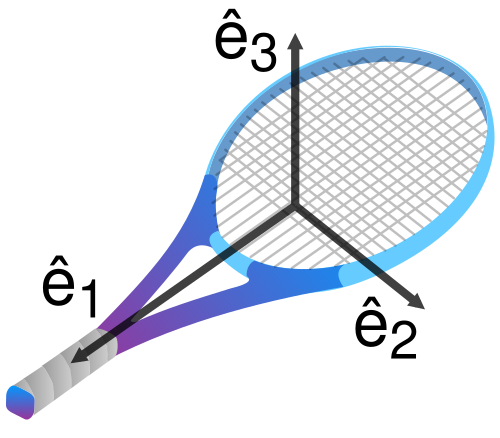
\includegraphics[width=0.6\linewidth]{revistas/002/imaxes/Tennis_racquet.png}
    \captionof{figure}{Eixos principais dunha raqueta de tenis.}
    \label{fig:raqueta}
\end{centering}\vspace{10pt}

No noso día a día podémolo visualizar facilmente, por exemplo, se colles o teu
tubo de pasta de dentes, o agarras dende o lado oposto á tapa (co logo cara
arriba) e o lanzas sobre sí mesmo, se tes a maña necesaria (moita) para volvelo
agarrar, verás que agora está boca abaixo. Este fenómeno é moito máis visible
nas raquetas de tenis, de aí o seu nome. Un posible efecto secundario é que o
coñecedor do fenómeno vai pasarse unha semana lanzando obxectos co fin de
comprobalo, e co fin de evitalo, imos tentar explicar a física do asunto.


\subsection*{A física do fenómeno: Por que?}

Co obxectivo de explicar o porque deste fenómeno temos que desempolvar os nosos
apuntamentos de Mecánica Clásica II e recordar que o movemento xiratorio dun
obxecto (sólido ríxido en términos físicos) depende principalmente da dirección
en que xiremos o corpo e o ``esforzo'' que supón manter a rotación neste eixo.
É dicir, custa menos enerxeticamente xirar un cilindro sobre o seu eixe axial
que se o xiramos sobre un eixe perpendicular a este coa mesma velocidade
angular. As ferramentas matemáticas que nos dan esta información son o vector
de velocidade angular ($\vec{\omega}$) e o tensor de inercia ($\mathbb{I}$).
Pero aínda queda a parte máis importante: obter o movemento do obxecto (as
ecuacións do movemento), que se conseguen unha vez se resolvan as ecuacións de
Euler que relacionan as compoñentes da velocidade angular e do tensor de
inercia (tamén chamados momentos de inercia) nun determinado sistema de
referencia. Como estamos a traballar nun espazo de 3 dimensións, as compoñentes
da velocidade angular e momentos de inercia tamén serán 3, por simplicidade:
$\omega_1, \omega_2, \omega_3$ e $I_1, I_2, I_3$.\\

En principio, este sistema de ecuacións diferenciais pode ser sinxelo de
resolver se o obxecto é moi simétrico, pero este non é o caso da porca ou da
raqueta de tenis, polo que temos que esforzarnos máis para obter información
destes movementos. Como xa adiantamos anteriormente, se consideramos un xiro
maioritario nun dos eixos principais e xiros minoritarios nos outros eixos,
chegamos a que as ecuacións de Euler nos din que o movemento naquel eixo
principal asociado ao momento de inercia intermedio ($I_1>I_2>I_3$, por
exemplo) é inestable, feito que explica a aparición do efecto Dzhanibekov.
\textit{Pero entón non temos unha solución analítica para o movemento?} Si
existen, o problema é que involucran ferramentas matemáticas máis profundas,
como as funcións elípticas de Jacobi \cite{RouthDynamics} ou o elipsoide de
Poinsot \cite{VanDamme2017}, polo que non imos entrar en detalles.

\subsection*{Aplicacións e consecuencias: Apocalipse?}

Unha das razóns polas que o goberno soviético ocultou este fenómeno foi
principalmente polo medo a que a Terra, ao ser un corpo que non é perfectamente
simétrico, puidese sufrir este mesmo efecto, o que, evidentemente, sería
catastrófico. Non obstante, a masa da Terra está disposta tal que xira sobre o
seu eixo de menor inercia e polo tanto, de forma estable, evitando a
apocalipse. Igual que coa Terra, ocorre o mesmo cos demais planetas, polo que é
xusto preguntarnos por que os planetas xiran sobre o seu eixo de menor inercia
e isto é consecuencia directa da conservación do momento angular herdado do
disco protoplanetario que formou o Sistema Solar. Aínda así, detectáronse unha
serie de lúas orbitando aos planetas gaseosos que si amosan este efecto e, máis
interesante aínda, publicouse recentemente que unha variedade de púlsar chamado
magnetar tamén pode sufrir este mesmo efecto por culpa do seu campo magnético
extremo e provocar ondas gravitacionais \cite{Kantor2023}. Finalmente, tamén se
teorizou coa posibilidade de empregar este efecto para a construción de naves
que aproveiten o fenómeno para cambiar o sentido da viaxe, o que reduciría
considerablemente o peso e o combustible necesario para estas misións
\cite{Ono2022}.

\printbibliography

\end{multicols}
\end{refsection}
